%
% LUMOS DOCUMENTATION: USER'S GUIDE
% $Header: /tmp/cvsroot/lumos/docs/lumos-user-guide.tex,v 1.2 2009-01-23 16:33:29 steve Exp $
%
% Copyright (c) 2009, 2011, 2012 by Steven L. Willoughby, Aloha,
% Oregon, USA.  All Rights Reserved.  Licensed under the Open Software
% License version 3.0.
%
% This product is provided for educational, experimental or personal
% interest use, in accordance with the terms and conditions of the
% aforementioned license agreement, ON AN "AS IS" BASIS AND WITHOUT
% WARRANTY, EITHER EXPRESS OR IMPLIED, INCLUDING, WITHOUT LIMITATION,
% THE WARRANTIES OF NON-INFRINGEMENT, MERCHANTABILITY OR FITNESS FOR A
% PARTICULAR PURPOSE. THE ENTIRE RISK AS TO THE QUALITY OF THE ORIGINAL
% WORK IS WITH YOU.  (See the license agreement for full details, 
% including disclaimer of warranty and limitation of liability.)
%
% Under no circumstances is this product intended to be used where the
% safety of any person, animal, or property depends upon, or is at
% risk of any kind from, the correct operation of this software or
% the hardware devices which it controls.
%
% USE THIS PRODUCT AT YOUR OWN RISK.
% 
% 
\documentclass{article}
%\usepackage[dvips]{graphicx}
\usepackage{graphicx}
\usepackage{epsfig}
\usepackage{textcomp}
\begin{document}
\title{Lumos User's Guide}
\author{Steve Willoughby}
\date{4 December 2011 \\ For Lumos Verison 0.5}
\maketitle
\tableofcontents
\pagebreak
\vfill
\begin{flushleft}
Document revision 0.5, 4 December 2011;
for software version 0.5.

Copyright \copyright\ 2009, 2011, 
(Software described \copyright\ 2005--2008, 2011) by
Steven L.\ Willoughby,
Aloha, Oregon, USA.  All Rights Reserved.


This document is part of the Lumos Light Orchestration System software package, distributed under the terms and conditions of the Open Software License, version 3.0.  For full details, see the file ``{\tt LICENSING}'' distributed with Lumos, or go to {\tt http://www.opensource.org}.
\end{flushleft}
\pagebreak

\section{Introduction}
Lumos is an open-source, platform-independent software system which
orchestrates light displays.  A typical application for Lumos is to control
complex Christmas light arrangements.  These displays consist of
pre-programmed sequences of circuit output changes (on, off, and various
dimmer levels), either as stand-alone patterns or synchronized to music.

Lumos is still a work in progress.  This document describes version 0.5, which
is an ``alpha'' level release with less functionaity than ultimately planned,
and not fully tested.  It is provided in this pre-release state for evaluation 
and experimentation purposes while the implementation of the remainder is 
being completed.

Lumos is also a class library which provides a framework for applications
to control SSRs and similar devices.  The included Lumos software (for creating,
editing, and playing back sequences for such things as synchronized 
Christmas light displays) is one example of an application suite using this
framework.  Others exist and may yet be written in the future.  For example,
the author also created a software package for running game show events,
with a computer-generated game board, control over contestant buttons and
displays, scoreboards, as well as control over stage lighting effects
in sync with the game board effects.  This application incorporates the
Lumos class library, and uses it to communicate with the various hardware
devices involved in those productions.

\subsection{Warning and Disclaimer}
This product is provided for educational, experimental or personal
interest use, in accordance with the terms and conditions of the
aforementioned license agreement, ON AN ``AS IS'' BASIS AND WITHOUT
WARRANTY, EITHER EXPRESS OR IMPLIED, INCLUDING, WITHOUT LIMITATION,
THE WARRANTIES OF NON-INFRINGEMENT, MERCHANTABILITY OR FITNESS FOR A
PARTICULAR PURPOSE. THE ENTIRE RISK AS TO THE QUALITY OF THE ORIGINAL
WORK IS WITH YOU.  (See the license agreement for full details, 
including disclaimer of warranty and limitation of liability.)

Under no curcumstances is this product intended to be used where the
safety of any person, animal, or property depends upon, or is at
risk of any kind from, the correct operation of this software or
the hardware devices which it controls.

{\bf USE THIS PRODUCT AT YOUR OWN RISK.}

\subsection{Supported Platforms}
Lumos is being developed on the Linux platform.
It is being developed in a platform-neutral manner and is expected to run on
most current platforms, including Linux, Unix, MacOS~X, and Windows.  It has
been tested and works successfully on Windows~XP, Windows~7, Ubuntu Linux 8.10--11.10,
and FreeBSD 8.2.

\subsection{Supported Hardware}
Lumos includes hardware device drivers for the following circuit controllers:
\begin{description}
 \item[FireGod:] Popular DIY solid-state relay controller capable of
  controlling 32 output channels with dimmer capability.
  {\em (Interface: serial; Status: untested)\/}
 \item[Olsen~595:] Another popular DIY SSR controller, capable of controlling
  a set of output channels (Lumos assumes 64 by default).
  {\em (Interface: parallel; Status: Under development; not yet ready for use.)\/}
 \item[Grinch:] We believe the Grinch DYI SSR controller has a compatible
  command protocol with the Olsen~595, so Grinch users should be able to use
  the Olsen~595 driver for them.
 \item[Renard:] Yet another popular DIY SSR controller which can be built
  to control 8, 16, 24, 32, or 64 channels with dimming capability.
  {\em (Interface: serial; Status: untested.)\/}
 \item[Lumos:] A custom-designed SSR controller by the author of Lumos, 
  capable of controlling 48 output channels with dimming capability.\footnote{Previously,
  this was referred to as ``48SSR'' or ``SSR48'' until the name Lumos was settled upon.
  The Lumos software accepts the legacy name ``{\tt 48ssr}'' for this unit, but that
  will eventually be deprecated.  The name ``{\tt lumos}'' should be used instead.}
  {\em (Interface: serial; Status: tested OK.)\/}
 \item[X-10~CM17a:] Also known as the ``Firecracker,'' sends commands via 
  built-in RF transmitter to an X-10 receiver module.  Each controlled device
  requires an individual X-10 module.  Current load capacity, dimming
  capability and other parameters vary for each individual X-10 module used.
  {\em (Interface: serial; Status: Under development; not yet ready for use.)\/}
 \item[LynX-10:] Another X-10 computer interface like the Firecracker, but
  directly wired into the power system via an X-10 TW523 module or equivalent
  instead of sending RF signals.  It is also a more intelligent unit with a
  faster communications protocol.  However, all the same caveats and
  restrictions inherent to X-10 systems apply.  Generally, the direct SSR
  controllers will give better results for fast-changing, synchronized
  lighting sequences than X-10.
  {\em (Interface: serial; Status: Under development; not yet ready for use.)\/}
\end{description}


\subsection{Extensibility}
Extending the {\tt Lumos.Device.ControllerUnit}
base class may be done to create new device drivers for Lumos.
Knowledge of Python programming is required.  See the
``HACKING.pdf'' document and manual page entries ``lumos-controller(4)''
and ``lumos-network(4)'' for more details.

\subsection{Glossary of Components}
A Lumos-managed light show consists of the following components.  The
remainder of this document will be devoted to a description of how they
interact, so understanding these basic terms will be helpful for understanding
what follows.

\subsubsection{Hardware}
\begin{description}
	\item[Power source:]
 		A supply circuit providing power to run the lights.  Each individual
		circuit breaker is identified in Lumos as a named ``power source''
		to help plan the show's current load.  By organizing your show with
		this in mind, you can work to avoid overloading any circuits on
		your breaker panel.
	\item[Controller:]
		A device which takes commands from Lumos to change the output levels
		on its {\em channels\/}.  Often, the controllers are located outside
		near the lights which are plugged into their output channels.  They
		may alternatively be located in a central indoor location, with
		extension cords running out to the controlled loads.
	\item[Channel:]
		Each output circuit provided by a {\em controller\/} is referred to
		as a {\em channel.\/}
	\item[Network:]
		A communications interface provided to connect the PC running Lumos
		with a set of hardware controllers.  These come in four different
		types:
		\begin{description}
			\item[Serial:]
				Plugged into a serial port on the PC, sending 8-bit bytes
				serially over RS-232 or RS-485 (or some other sort of serial
				hardware protocol) to a set of one or more {\em
				controllers.\/}  Whether one or many controllers may exist
				on the same serial network depends on the type of controllers
				involved.  Ones which have individual addresses assigned to
				them can share a serial network with other controllers of the
				same make (i.e., their serial protocols must be 100\%
				compatible in order for commands addressed to one to not
				confuse the others).  
				Examples of controllers using this type of network include the
				FireGod (up to 4 per network), 
				Lumos (up to 16 per network), 
				LynX-10 (one per network),
				and the 
				Renard (up to 128 per network).
			\item[Serialbit:]
				(Short for ``serial, bit-at-a-time'' network.)  Technically, 
				all serial networks are bit-at-a-time, but rather than the
				usual asynchronous scheme of transmitting an entire word of
				bits over the TxD line, this type of network employs
				synchronous bit-at-a-time transfers by manipulating the serial
				port's control lines rather than the data lines.  It might be
				possible to connect a serial and serialbit network to the same
				PC serial port, but this is not recommended and not verified
				to work.  Only one controller at a time can usually be 
				connected to a serialbit network.
				%Examples of controllers using this type of network include the
				One example controller using this type of network is the
				Firecracker (X-10 CM17a).
			\item[Parallel:]
				Full eight-bit parallel data transfer to connected
				controllers.
				Currently no known controllers use this type of network.
			\item[Parbit:]
				Synchronous bit-at-a-time data transfer in a manner similar
				to the serialbit network type, but using the control signal
				lines of the PC's parallel port instead of the serial port.
				Examples of controllers using this type of network include the
				Olsen 595 and Grinch.  Only one controller at a time may be
				attached to the parbit network, typcially (but this depends
				more on the controller device than the network).
		\end{description}
	\item[Loads:]
		The lights or other devices controlled by the controllers.
\end{description}

\subsubsection{Configuration and Data}
The following data sets provide the necessary context and programming
information for Lumos to perform your show using the hardware devices
connected to it:

\begin{description}
	\item[Show configuration:]
		Lumos uses a show configuration file to describe all the hardware
		elements in play.  This file is described in detail in the manual page
		``lumos-config(5).''
	\item[Sequence:]
		A programmed sequence of on/off and dimmer level change events
		to be sent to the various controllers managed by Lumos.  Each 
		sequence is stored in a text file as described in the manual page
		``lumos-sequence(5).''
	\item[Scene:]
		A collection of one or more sequences which together comprise a
		complete individual scene (such as one song) from the point of view of
		the audience.
	\item[Show:]
		The full set of scenes, hardware, and everything comprising a single
		instance of your display.  For example, ``Our Christmas Lights for
		2009'' might be a show, which contains scenes such as the song ``God
		Rest Ye Merry, Gentlemen'' which includes sequences such as
		``mega-tree light chasing pattern''.
\end{description}

\subsubsection{Software}
The following Lumos software components are available for use to accomplish
the creation and playback of the scenes in your light show.
\begin{description}
	\item[lcheck:]
		A utility to check a show configuration file for basic errors.
	\item[lplay:]
		Plays (or performs) a list of sequence files on the hardware
		configured for a show.
	\item[vixen2lumos:]
		An import utility to assist with using Lumos to play sequences
		previously created with the Vixen light control program.
\end{description}

\subsection{Licensing Information}
Lumos is a copyrighted work, distributed under the terms and conditions of the 
Open Software License version 3.0.  See the ``LICENSE'' file which accompanied
the software distribution for full details, or see www.opensource.org.

\subsection{The Name of the Game}
``Lumos'' is an acronym of {\em lumen,\/} the Latin word for ``light,'' and
the initial letters of ``orchestration'' and ``system.''  Hence, ``Light
Orchestration System.''

\section{Setting Up a Show}
Your show planning begins before doing anything with the Lumos software.
First, look at the area you'll be lighting as something of a ``canvas'' and
think of what lighting effects you wish to create in that space.  Keep in mind
what resources you have available, including not only what lights you have on
hand to install, but also how many amps of available power you have to supply
it.  Think of what music you might want to play with it (if any), and what
general mood you wish to create in each scene.

Once you have an idea what you will be accomplishing, sketch out the location
of all the lights and other devices, and start assigning them to controllers.
You'll want to keep in mind where you want the controllers to be located, and
how many amps they'll be supplied, when assigning loads to their output
channels.

Having done that, you'll need to create the Lumos show configuration file to
describe your hardware setup.  For the simple example we'll walk through in
this tutorial, we will be lighting up a tree in three colors of lights, which
will be controlled on channels 10, 11, and 12 of a FireGod controller.
Additionally, we have red and green floodlights which already happen to be
rigged up to X-10 dimmer modules (on addresses ``C2'' and ``C5'' respectively),
so we'd like to control those as well.
We have a LynX-10 computer interface to communicate with our X-10 home
automation system.

A future release of Lumos is expected to have a convenient GUI interface for
managing show configuration profiles, but at present, setting up the show
configuration involves editing a text file.  The format is easy to edit,
however, so this shouldn't prove too difficult.  You will need to use a text
editor which will produce plain ASCII files (such as vi, EMACS, or Notepad).

You can call the file anything you like, although the name should be
descriptive of the show.  For best results, the file name should not contain
spaces or special characters which would require quoting or escaping to use in
command lines.  By convention, the show configuration files have a suffix of
``{\tt.conf}'' but this is not required.

To begin, we create a {\tt[show]} section describing the basic elements of the
show.  We'll begin by giving the title and description of the show itself.
This section also includes a list of all the power sources and communications
networks we'll be using.

In our case, the FireGod controller will be plugged into a 20A outdoor plug on
circuit breaker \#15 on our panel.  The floodlights are wired to the 15A
circuit on breaker \#22B.

The FireGod and LynX-10 will be on separate serial ports, named ``tree'' and
``floods,'' respectively.

\begin{figure}[htbp]
\begin{verbatim}
[show]
title=A Minimal Light Show
description=Just an example for the tutorial.
powersources=15 22b
networks=tree floods
\end{verbatim}
\caption{Sample {\tt[show]} Section}
\label{conf:show}
\end{figure}

Figure~\ref{conf:show} shows the configuration file section which informs 
Lumos of what was just described in these paragraphs.

Note that there are more details about each of these elements, but we'll
describe them individually in their own sections.  This just lets Lumos know
what elements exist.  Also note that the list of power sources and networks
are separated by spaces in these values.  We could have named them anything we
wanted.  We chose ``15'' and ``22b'' because they matched the labels on the
circuit panel, and the names ``tree'' and ``floods'' because they were
reasonably descriptive.  The names chosen should contain just letters, digits,
and underscores (``\verb+_+'') for best results.

Next, we'll describe the power sources themselves.  There are only two things
Lumos needs to know about each power source: the current load capacity it
offers {\em to the light show\/} (i.e., if a power circuit has other loads, be
sure to account for them before telling Lumos how much available current it
has on that circuit), and whether that circuit is protected by GFCI circuit
breakers.

{\bf Important safety note: Providing this information to Lumos does not
guarantee it will not overload anything!  You are still able to define a
sequence which would overload your panel if you choose to do so!  These values
in the configuration are intended to be a helpful guide to yourself when
planning your show.  Do not rely on Lumos to ensure your show stays within
safe operating parameters.  That's not its function.}

\begin{figure}[htbp]
\begin{verbatim}
[power 15]
amps=20
gfci=yes

[power 22b]
amps=15
gfci=yes
\end{verbatim}
\caption{Sample {\tt[power...]} Sections}
\label{conf:power}
\end{figure}

In Figure~\ref{conf:power} we add two new sections to our configuration file,
each to define the specific attributes of one of the power sources mentioned
in the {\tt powersources} line of the {\tt[show]} section.  Note that the
section names include the power source names we invented earlier.

Now we need to define the particulars for the networks ``tree'' and ``floods''
we mentioned in the {\tt networks} line of the {\tt[show]} section.  These are
both traditional serial networks, so we'll need to specify such parameters as
baud rate and so forth for each one.  We will also list which controllers are
plugged into each network here, although the specifics about those controllers
will be explained later in their own sections.

Figure~\ref{conf:nets} shows the two new sections added to the configuration
file to describe these networks.  We made up the names ``{\tt fgtree}'' to refer to
our FireGod SSR controller directing the lights on our tree, and
``\verb+home_auto+'' to refer to the home automation X-10 interface (the LynX-10
unit).

\begin{figure}[htbp]
\begin{verbatim}
[net tree]
description=serial net for FireGod on the tree
units=fgtree
type=serial
port=0
baudrate=9600

[net floods]
description=flood lights on X-10 control
units=home_auto
type=serial
port=1
baudrate=1200
\end{verbatim}
\caption{Sample {\tt[net...]} Sections}
\label{conf:nets}
\end{figure}

The controller units themselves are now each defined in a new section which
defines the type of controller used, along with any specific parameters
required by that controller.

The list of controllers supported by this version of Lumos is summarized in
Table~\ref{conf:controllers}.  

\begin{table}[htbp]
\begin{center}
\begin{tabular}{|l|l|l|l|}\hline
\bf Type   & \bf Network   & \bf Channels & \bf Extra Parameters \\\hline\hline
cm17a      & serialbit     & A1--P16      & {\it(none)}\\\hline
firegod    & serial        & 0--31        & address, channels\\\hline
lumos      & serial        & 0--47        & address\\\hline
lynx10     & serial        & A1--P16      & {\it(none)}\\\hline
olsen595   & parbit        & 0--63*       & channels\\\hline
renard     & serial        & 0--63*       & address, channels\\\hline
\end{tabular}
\end{center}
*(or the highest channel number actually implemented on the controller.)
\caption{Supported Controller Types}
\label{conf:controllers}
\end{table}

In our case, we need to add a section for the FireGod controller (shown in
Figure~\ref{conf:fgtree}).  In the {\tt[net~tree]} section, we chose to refer 
to this particular controller as ``{\tt fgtree},'' so the details for this
controller unit are described in a section called ``{\tt[unit fgtree]}.''

\begin{figure}[htbp]
\begin{verbatim}
[unit fgtree]
type=firegod
address=0
power=15
\end{verbatim}
\caption{Sample {\tt[unit fgtree]} Section}
\label{conf:fgtree}
\end{figure}

There are a couple of things to note on this section.  Each 
``{\tt[unit...]}'' section requires at least two lines: ``{\tt type},'' which
should be one of the type names listed in Table~\ref{conf:controllers}, and 
``{\tt power},'' which is the name of the power source this unit feeds from.
In this case, this FireGod controller is plugged into circuit 15 from our
breaker panel (described above in the {\tt[power~15]} section).

According to Table~\ref{conf:controllers}, a FireGod controller also needs two
additional fields: ``{\tt address},'' which we specify here as 0, and 
``{\tt channels},'' which is the number of channels the unit supports (since 
not every FireGod controller may be built with the same number of outputs).
Note that in this example we did {\em not\/} include this line, so Lumos
assumes the default value of 32 channels.

We will also add a \verb+[unit home_auto]+ section for the X-10 lights (see
Figure~\ref{conf:x10}).

\begin{figure}[htbp]
\begin{verbatim}
[unit home_auto]
type=lynx10
power=22b
\end{verbatim}
\caption{Sample {\tt[unit~home\_auto]} Section}
\label{conf:x10}
\end{figure}

Finally, we need to specify what loads are plugged into each output channel.
Each of these is described in a section named with the controller unit name
and channel name.  For example, the output channel \#10 of our FireGod
controller unit would be described in a section called {\tt[chan~fgtree.10]}.
Figure~\ref{conf:fgtree10} shows the channel definitions for the outpus from
this controller.

\begin{figure}[htbp]
\begin{verbatim}
[chan fgtree.10]
name=Tree, red
load=.3
dimmer=yes

[chan fgtree.11]
name=Tree, green
load=.3
dimmer=yes

[chan fgtree.12]
name=Tree, blue
load=.3
dimmer=yes
\end{verbatim}
\caption{Sample {\tt[chan fgtree...]} Sections}
\label{conf:fgtree10}
\end{figure}

For each output channel, we specify a descriptive name for the output, the 
load in amps, and whether Lumos should try to dim that load.

For the flood lights defined as shown in Figure~\ref{conf:homeauto}, we want
to keep the lights warm all the time, so we add one more line to each of their
sections: ``{\tt warm=10}.''  This means that the output for those channels
should never go below 10\% regardless of what any sequence specifies.

\begin{figure}[htbp]
\begin{verbatim}
[chan home_auto.C2]
name=Flood, red
load=1
dimmer=yes
warm=10

[chan home_auto.C5]
name=Flood, green
load=1
dimmer=yes
warm=10
\end{verbatim}
\caption{Sample {\tt[chan home\_auto]} Sections}
\label{conf:homeauto}
\end{figure}

We'll save this data into a file called {\tt myshow.conf}, and run the {\tt
lcheck} utility to check for errors in the file.  (Of course, a program such
as {\tt lcheck} can't check for {\em everything,\/} so please also exercise
due dilligence in creating a correct configuration file, too.)

\begin{verbatim}
$ lcheck myshow.conf
ValueError: Address 0 out of range for a FireGod SSR Controller Module
\end{verbatim}

This uncovered an error we inadvertently made:  FireGod controllers use
addresses in the range $1\le x\le4$, so there can't be a unit \#0.
We'll edit the {\tt[unit~fgtree]} section to read ``{\tt address=1}''
instead and re-run the check utility:

\begin{verbatim}
$ lcheck myshow.conf
\end{verbatim}

Now at least {\tt lcheck} is happy with the file.  It could also be useful to
re-run this program with the {\tt --verbose} option.  This produces a text 
summary of the show configuration, which is convenient to refer to when wiring
up the hardware or working with your sequences:

\begin{verbatim}
$ lcheck --verbose myshow.conf
SHOW DESCRIBED BY FILE 'myshow.conf':
 Title: A Minimal Light Show
 Description: Just an example for the tutorial.
-------------------------------------------------------------
 POWER SOURCES:
  15            20A [GFCI]
  22b           15A [GFCI]
-------------------------------------------------------------
 COMMUNICATIONS PARAMETERS
  NETWRK PORT  SPEED BPSXR DESCRIPTION
  floods    1   1200 8n1-- flood lights on X-10 control
  tree      0   9600 8n1-- serial net for Firegod on the tree
-------------------------------------------------------------
 DEVICE CONTROLLERS:
  NETWRK UNIT     POWER DESCRIPTION
  floods home_auto  22b LynX-10/TW523 Controller
  tree   fgtree      15 FireGod SSR Controller (32 channels), module #1
--------------------------------------------------------------
 DEVICE CHANNELS:
  UNIT     CHAN POWER LOAD D WARM DESCRIPTION
  home_auto  C2 22b     1A D   6% Flood, red
  home_auto  C5 22b     1A D   6% Flood, green
  fgtree     10 15    0.3A D   0% Tree, red
  fgtree     11 15    0.3A D   0% Tree, green
  fgtree     12 15    0.3A D   0% Tree, blue
--------------------------------------------------------------
 POWER LOAD SUMMARY:
  15         Loaded to   4%
  22b        Loaded to  13%
Total allocated load: 2.9 Amps
\end{verbatim}

See the manual entry for ``lumos-config(5)'' for full details about the
configuration file's format and contents.

We're now ready to start defining sequences for our show.

\section{Creating a Sequence}
Sequences are stored in simple text files which describe each output
channel change event in the show, and when that event is scheduled to
occur.  

Lumos will ultimately include a GUI scene editing tool which will allow for
easy creation of sequences, previewing them, editing them, and synchronizing
them to music.  In this pre-release state, however, that functionality does
not yet exist.

This leaves us with two options, then, in the mean time.  We can create 
sequence files manually, or we can import sequences from another tool.

\subsection{Manual Creation of Sequence Files}
The sequence file format is fairly simple to understand, and therefore 
creating one in a text editor is quite possible.  The problem with attempting
to do this is simply that a typical sequence has such a high number of events,
this can be an overwhelmingly tedious task.

For testing Lumos or experimenting with it, however, this approach may still
be useful.  The full details for this file format are documented in the manual
entry for ``lumos-sequence(5)''.

We'll manually create a sequence file now which will define the following
sequence of events:
\begin{description}
	\item[00:00.0]
		Start fading up the red flood lights (over 2 seconds)
	\item[00:01.0]
		Turn on red lights in the tree
	\item[00:05.0]
		Flash the red, green, and blue lights in sequence for 1/10 second
		each.
	\item[00:05.8]
		Turn off the tree lights.
	\item[00:06.0]
		Crossfade flood lights to green over 2 seconds.
	\item[00:07.0]
		Turn on the tree red at 1/2 brightness.
	\item[00:10.0]
		Fade everything to black over 1.5 seconds.
\end{description}

Sequence files use a basic comma-separated value (``CSV'') format.  Each 
line of the file is a ``record'' which describes a single distinct aspect
of the sequence.  These records are themselves divided into ``fields'' which
are separated from each other by commas.  The first field in each record
determines what type of record it is.

A sequence file always begins with the record ``{\tt V3}'' to indicate this is a
version 3 Lumos sequence file.  

Following this is a set of controller unit
definition records describing the controllers used by this sequence.  
The initial field of each of
these  is ``{\tt U}''; the remaining fields give the controller name as 
defined in the
show configuration, followed by a list of the output channels used in this
sequence.  Figure~\ref{seq:u}
shows the first three lines of our sequence file, indicating the controller
units we'll be using.

\begin{figure}[hbtp]
\begin{verbatim}
V3
U,fgtree,10,11,12
U,home_auto,C2,C5
\end{verbatim}
\caption{Sequence File: Controller Unit Definitions}
\label{seq:u}
\end{figure}

From here on, we add a ``time'' record to indicate when in the sequence
the following set of events will take place, then the events themselves, and
so on.  

Time records consist of the letter ``{\tt T}'' followed by a number
of milliseconds from the beginning of the sequence.  

Event records describe what takes place at any given point in time.  The
current version of Lumos uses just one type of event, described in an ``{\tt
E}'' record.  These have four additional fields: the controller unit number,
channel number, value to set the output channel to, and the number of
milliseconds over which to effect that change in level.  The unit and channel
numbers are numbered starting with 0 for the first unit listed in the sequence
file, and starting with 0 for the first channel listed for any given
controller.

This means that given our unit definition for this file:
\begin{verbatim}
U,fgtree,10,11,12
U,home_auto,C2,C5
\end{verbatim}
we have the following assignment of unit and channel numbers for use within
this sequence file:
\begin{center}
\begin{tabular}{|r|r|l|}\hline
\bf Unit \# & \bf Channel \# & \bf Configuration ID \\ \hline\hline
0 & 0 & \tt fgtree.10 \\ \hline
0 & 1 & \tt fgtree.11 \\ \hline
0 & 2 & \tt fgtree.12 \\ \hline
1 & 0 & \tt home\_auto.C2 \\ \hline
1 & 1 & \tt home\_auto.C5 \\ \hline
\end{tabular}
\end{center}

So our first event, at time 00:00.000, which fades the red flood lights
(controller 1, channel 0) to 100\% over 2 seconds (2,000 milliseconds)
would be entered as:
\begin{verbatim}
T,0
E,1,0,100,2000
\end{verbatim}
Then, at 00:01.000, we turn on the red tree lights (controller 0, channel 0)
to 100\% instantly:
\begin{verbatim}
T,1000
E,0,0,100,0
\end{verbatim}
At 00:05.000, we start cycling through controller 0's channels 0--2 at
0.100-second intervals:
\begin{verbatim}
T,5000
E,0,0,0,0
E,0,1,100,0
T,5100
E,0,1,0,0
E,0,2,100,0
T,5200
E,0,2,0,0
E,0,0,100,0
...
\end{verbatim}

The full text of the sequence file is shown in Figure~\ref{seq:all}.

\begin{figure}[p]
\begin{verbatim}
V3
U,fgtree,10,11,12
U,home_auto,C2,C5
T,0
E,1,0,100,2000
T,1000
E,0,0,100,0
T,5000
E,0,0,0,0
E,0,1,100,0
T,5100
E,0,1,0,0
E,0,2,100,0
T,5200
E,0,2,0,0
E,0,0,100,0
T,5300
E,0,0,0,0
E,0,1,100,0
T,5400
E,0,1,0,0
E,0,2,100,0
T,5500
E,0,2,0,0
E,0,0,100,0
T,5600
E,0,0,0,0
E,0,1,100,0
T,5700
E,0,1,0,0
E,0,2,100,0
T,5800
E,0,2,0,0
T,6000
E,1,0,0,2000
E,1,1,100,200
T,7000
E,0,0,50,0
T,10000
E,*,*,0,1500
\end{verbatim}
\caption{Sample Sequence File}
\label{seq:all}
\end{figure}

See the manual entry for ``lumos-sequence(5)'' for full details about this
file format.

If you wish, you can use a program which can edit CSV format files (e.g., a
spreadsheet).  Figure~\ref{seq:ss} shows our sequence file being edited in
Gnumeric (an open source spreadsheet program).

\begin{figure}[p]
%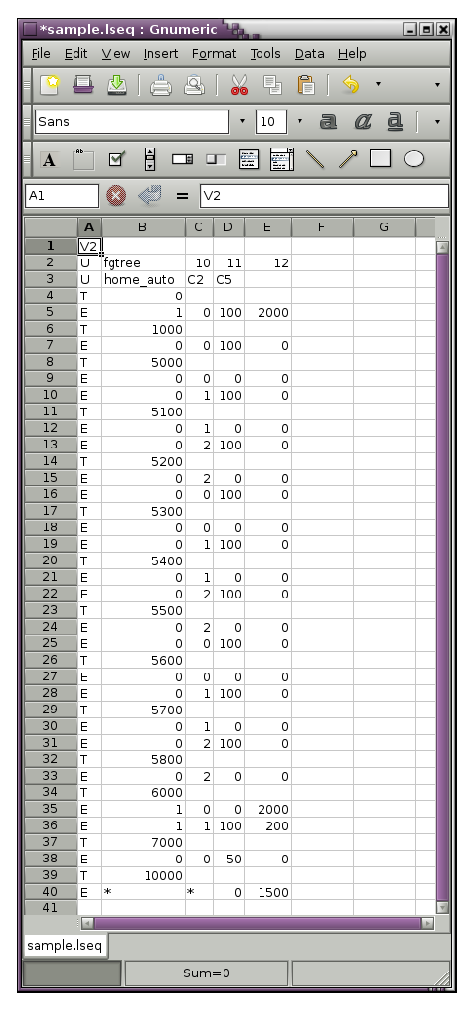
\includegraphics{seq-ss}
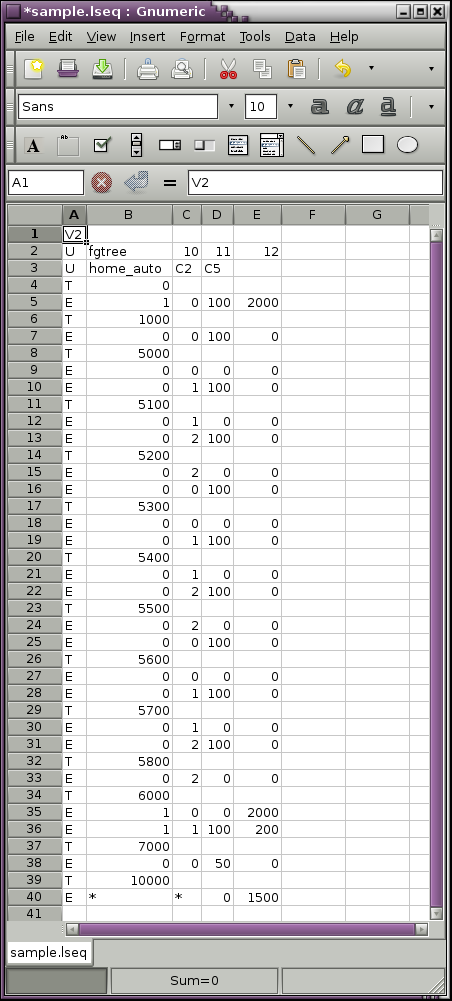
\epsfig{file=seq-ss.png, height=\textheight}
\caption{Sequence File in Spreadsheet Editor}
\label{seq:ss}
\end{figure}

\subsection{Importing Sequences from Vixen}
An alternative way of creating Lumos sequence files is to import them from
another program.  This can be especially convenient during the period before
Lumos' own GUI sequence editor is released.  Currently Lumos includes a simple 
import utility for the popular sequencing program Vixen.  

An imported sequence won't quite be the same as a native Lumos sequence,
though, due to the differences between how each system operates.  
Vixen, for example, handles events as individual snapshots capturing the state of every output channel at each instant in time. A typical device plug-in would just take that data and update every channel on each controller, regardless of whether they all changed state or just a single channel did. While several SSR controllers expect to be updated that way, not all do, and individually addressing the specific channels which change can be more efficient (depending on how much is being updated at one time). Lumos handles channel events separately so the choice of whether to send complete device updates or individual channel changes can be made by each device driver as appropriate for the hardware it's driving.

This means that imported sequences including gradual dimmer level changes will
appear in Lumos as a series of discrete level-set events instead of one.  

The vixen sequence import utility, {\tt vixen2lumos}, is designed to convert
standard Vixen sequences.  

Note that the import works best when Vixen is set to a profile which uses an
actual device plug-in (i.e., not just a ``preview window'' plugin).  Using,
for example, the Renard driver works well:

\noindent%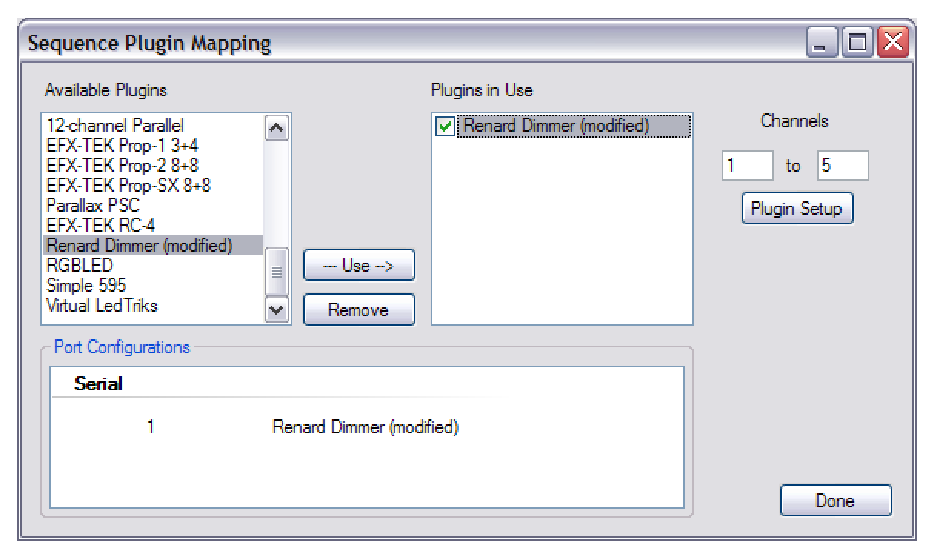
\includegraphics{vix-plugin}
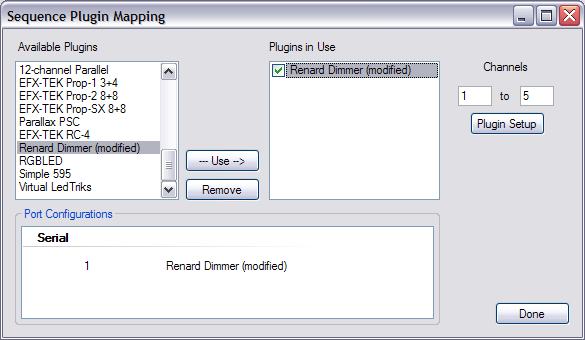
\epsfig{file=vix-plugin.png, width=\textwidth}

Create a profile which uses the set of output channels you need, select the
Renard plugin, and then define a new ``Vixen standard sequence'':

\noindent%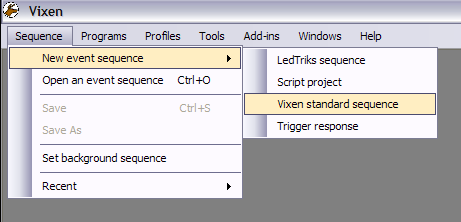
\includegraphics{vix-menu}
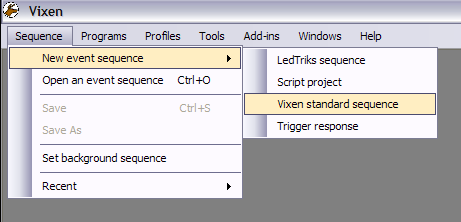
\epsfig{file=vix-menu.png, width=\textwidth}

Now proceed to build the sequence in Vixen as normal.  Figure~\ref{vix:seq}
shows the same sequence we discussed in the previous section, but created
using Vixen rather than by manual editing of the file.

\begin{figure}[p]
%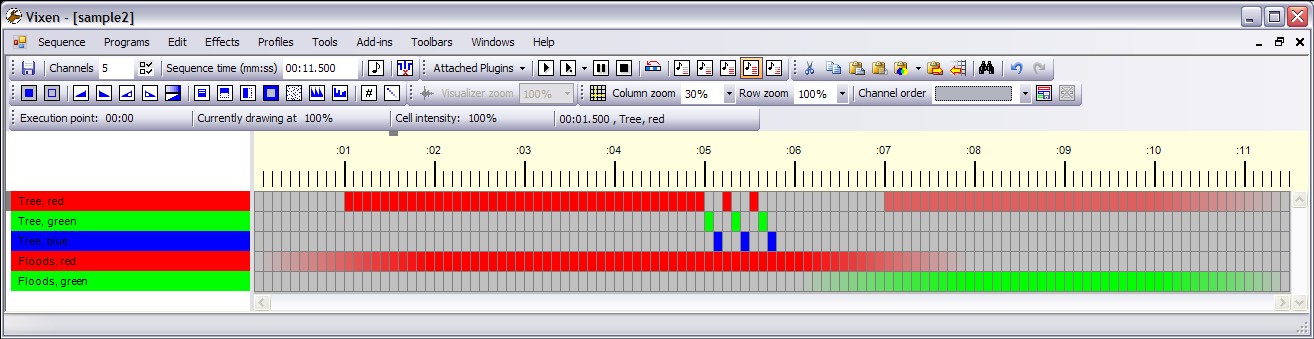
\includegraphics{vix-sequence}
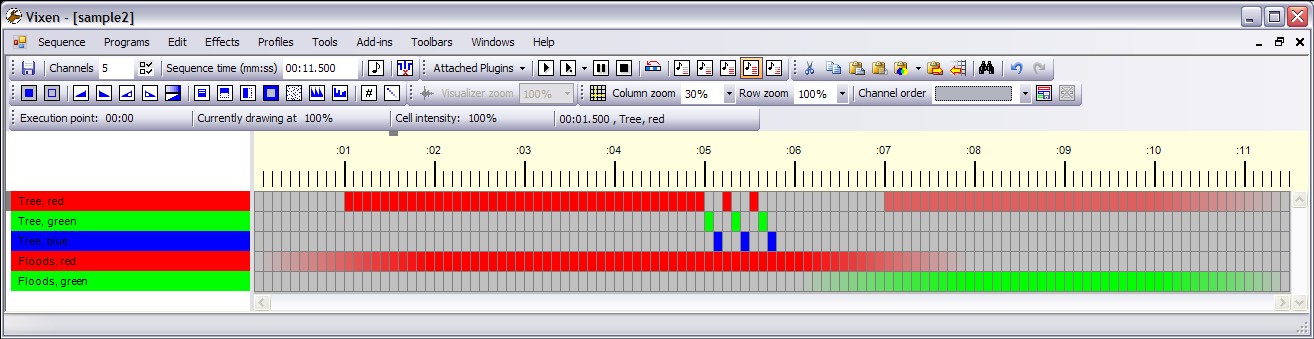
\epsfig{file=vix-sequence.png, width=\textwidth}
\caption{Sample Sequence in Vixen Editor}
\label{vix:seq}
\end{figure}

The saved sequence file (in our example, ``{\tt sample2.vix}'') can then be
imported into Lumos using {\tt vixen2lumos}.  The first step is to use the
{\tt --info} option to be sure the file is readable and that its general
parameters look close to what we'd expect.  This is just a simple sanity check
before we get too far:
\begin{verbatim}
$ vixen2lumos --info --input=sample2.vix
Loaded sequence data from Vixen:
  Duration:    00:11.500
  Value Range: 0 - 255
  Channels:    0
\end{verbatim}

If you see something like this (note the ``Channels:~0''), it means the
sequence file does not include the profile data.  Sometimes the combination of
plugins will pull this information into the sequence file, but if not, you can
ask Vixen to merge your profile data into the sequence.  Pull down the
``Profiles'' menu and choose ``Flatten profile into sequence,'' then save your
sequence again.

\noindent%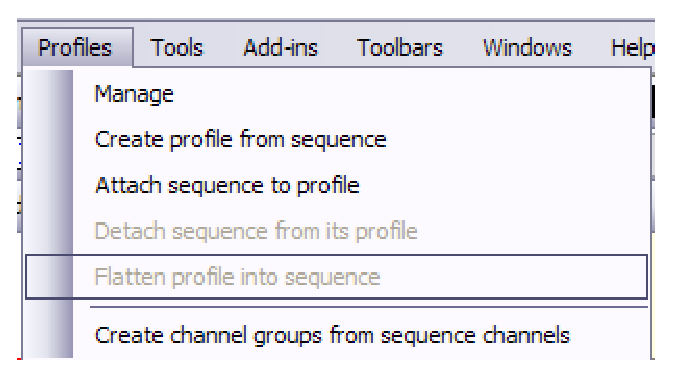
\includegraphics{vix-merge}
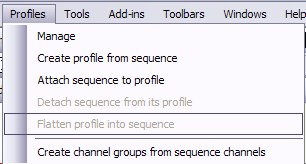
\epsfig{file=vix-merge.png, width=\textwidth}

Now re-check with the {\tt --info} option:
\begin{verbatim}
$ vixen2lumos --info --input=sample2.vix
Loaded sequence data from Vixen:
  Duration:    00:11.500
  Value Range: 0 - 255
  Channels:    5
    0 = "Tree, red"          RGB=FF0000 out=0
    1 = "Tree, green"        RGB=00FF00 out=1
    2 = "Tree, blue"         RGB=0000FF out=2
    3 = "Floods, red"        RGB=FF0000 out=3
    4 = "Floods, green"      RGB=00FF00 out=4
\end{verbatim}

That's better---we see the five channels we need, and the duration looks right.
Now we need to create a ``mapping file'' which tells Lumos which channels
defined in the Vixen sequence files correspond to which channels in the
Lumos show configuration.

The easiest way to do this is to let {\tt vixen2lumos} do most of the work
for us, by using the {\tt --genmap} option:
\begin{verbatim}
$ vixen2lumos --genmap=sample2.map --input=sample2.vix
\end{verbatim}
This will create a new file, {\tt sample2.map}, which is a list of the
channels found in the sequence file {\tt sample2.vix}.  The file contains
some comments describing the file and its contents, followed by these channel
map definitions:
\begin{verbatim}
0,"Tree, red",CONTROLLER,CHANNEL
1,"Tree, green",CONTROLLER,CHANNEL
2,"Tree, blue",CONTROLLER,CHANNEL
3,"Floods, red",CONTROLLER,CHANNEL
4,"Floods, green",CONTROLLER,CHANNEL
\end{verbatim}
We need to edit these to assign each of them to a Lumos controller and
channel name (as defined in our show configuration file):
\begin{verbatim}
0,"Tree, red",fgtree,10
1,"Tree, green",fgtree,11
2,"Tree, blue",fgtree,12
3,"Floods, red",home_auto,C2
4,"Floods, green",home_auto,C5
\end{verbatim}
See the manual entry for ``lumos-channel-map(5)'' for the full details on
this file and what can appear in it.

With this mapping in place, we are ready to convert the Vixen sequence to a
Lumos sequence file.  We do this by running the converter one last time:
\begin{verbatim}
$ vixen2lumos --input=sample2.vix --map=sample2.map \
    --conf=myshow.conf --output=sample2.lseq
\end{verbatim}
The sequence file {\tt sample2.lseq} can now be played in Lumos.

\section{Adding Audio Tracks to Sequences}
Each sequence may have an audio track attached to it.  The audio will begin playing
when the sequence begins running in {\tt lplay}.  If the audio is not finished playing
by the time the sequence ends, the audio playback will be stopped at that time.

To attach an audio file to a Lumos sequence, you need only add a single line to 
the sequence file:

\begin{verbatim}
A,test.ogg,100
\end{verbatim}

This will cause the audio file {\tt test.ogg} to play at 100\% volume level.  There are
other optional fields which may also be specified to control mono or stereo output,
sample frequency, sample bits, and buffer sizes, but these are not usually necessary
for you to adjust.  See the documentation in lumos-sequence(4) for full details.

Audio files attached to Vixen sequences imported via {\tt vixen2lumos} should generally
already have the file attachment record added for you to the sequence.  Make sure the
audio file itself is copied to the directory {\tt lplay} is reading from.

Many popular audio file formats are supported.  We recommend using OGG or WAV files.

\section{Checking Power Usage}
Before playing your sequences on real hardware, you should check to be sure
your sequence doesn't cause an overload on one of your circuits.  Ultimately,
your setup needs to be planned and put together by someone with adequate
understanding of electrical load management, and protected with circuit breakers
of the correct type to ensure your safety.  The Lumos system cannot guarantee
any particular situation \emph{won't} be hazardous, that's your responsibliity
as you arrange your show and the hardware involved.  However, the following 
procedure is a valuable tool to assist you in doing that.

The Lumos Power Meter utility {\tt lpower} will run through a set of sequence
files which you intend to play together as a scene, and calculate the power
consumed by that scene.  

To get a basic report, run:

\begin{verbatim}
$ lpower --conf=myshow.conf sample2.lseq
**NOTE**
The following circuit(s) had power draining at the end of the show.
If they remain on after the show, they will consume additional
power beyond what this report is showing.
This final power level was the end-state at the last instant of the
sequence, so is not figured into the calculations reported.

  0.13 amps on 22b
Total Runtime:      00:00:11.500 (11,500 mS)
Total Power Used:   0.000430 kWh

POWER SOURCE    PEAK (A)   AVERAGE (A)
15                  0.30       0.17412
22b                 1.87       0.94638
\end{verbatim}

The big warning message at the beginning of the report is letting us
know that after the scene is finished, some units were still drawing
power (either we left some of them running, or they have a ``warm''
setting which keeps a little power flowing into them at all times.
So we are aware that more power will continue being drawn if we leave
things as they are after the scene has concluded.
Specifically, circuit ``22b'' is still seeing a 0.13\,A load.

For the duration of our 11.5 second sequence, we consumed a very small
number of kilowatt-hours (less than one-thousandth), and we see what the
peak load was for every power supply circuit, as well as the average
current levels during the scene.

If we know how much we're paying for power, we can let {\tt lpower}
calculate an estimated price for the scene, as well.  Suppose we pay
6\textcent\ per kilowatt-hour:

\begin{verbatim}
$ lpower --conf=myshow.conf --price=0.06 sample2.lseq
.
.
.
Total Runtime:      00:00:11.500 (11,500 mS)
Total Power Used:   0.000430 kWh
Total Energy Cost: $0.0000 (~$0.00) @ $0.0600/kWh

POWER SOURCE    PEAK (A)   AVERAGE (A)
15                  0.30       0.17412
22b                 1.87       0.94638
\end{verbatim}

The cost for this little sequence turns out to be 0.0026\textcent,
which is rounded off to \$0.0000 in this report.\footnote{Actually, although Lumos shows the value with a dollar sign
in front of the value, any currency system will work.  You just indicate how many
``monetary units'' you are charged per kilowatt-hour, and the number of those units
Lumos estimates you'll be charged, down to 1/10,000 unit.}

{\bf Note:} Power rate schedules can be complex.  Lumos' {\tt lpower} utility is
not designed to predict your power bill with complete accuracy, but only to serve
as a basic guide for estimation purposes, primarily for circuit loading, not for
billing.

The {\tt lpower} program assumes as 120\,V line power voltage in its calculation
of kilowatt-hours.\footnote{It uses the simple formula of $P=I\times E$ to convert
amps ($I$) and volts ($E$) to watts ($P$).}  If your power is at a different voltage,
you can use the {\tt --volts} option, like so:

\begin{verbatim}
$ lpower --conf=myshow.conf --volts=110 sample2.lseq
.
.
.
Total Runtime:      00:00:11.500 (11,500 mS)
Total Power Used:     0.000394 kWh

POWER SOURCE    PEAK (A)   AVERAGE (A)
15                  0.30       0.17412
22b                 1.87       0.94638
\end{verbatim}

If you want a detailed description of exactly what power is being used by which
circuits at every instant during your scene, use the {\tt --graph-data} option, 
which will cause {\tt lpower} to dump a CSV file containing this information:

\begin{verbatim}
$ lpower --conf=myshow.conf --graph-data=sample2data.csv sample2.lseq
.
.
.
\end{verbatim}

We can then open the file {\tt sample2data.csv} in any program which understands
CSV (comma-separated value) files, including a spreadsheet program such as Microsoft
Office Excel, as shown in figure~\ref{csvexcel}.
\begin{figure}[htbp]
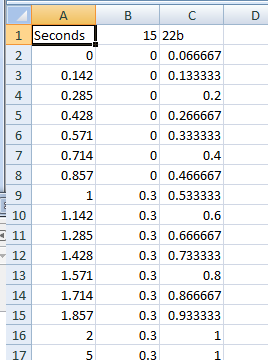
\epsfig{file=power-excel.png, width=.5\textwidth}
\caption{Power usage data in Excel\label{csvexcel}}
\end{figure}

The first column (``A'') is the elapsed time in the scene.  The other columns
are the amps drawn by each circuit starting at that point in time, continuing
on until the next event time (the next row of the spreadsheet).

Many programs can analyze this further.  For example, using Excel we can 
select ``Insert,'' ``Charts (Scatter),'' ``Scatter with straight lines,''
and a nice graph is produced showing our power usage, as shown in figure~\ref{csvgraph}.
The $x$ axis is in seconds, and the $y$ axis is in amps.
\begin{figure}[htbp]
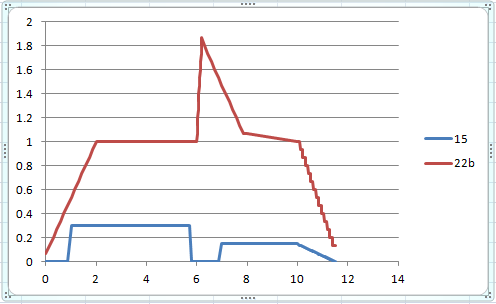
\epsfig{file=power-graph.png, width=\textwidth}
\caption{Power usage graphed in Excel\label{csvgraph}}
\end{figure}



\section{Performing (Playing Back) Sequences}
The playback function in Lumos is currently fairly simple, although much more
development and sophistication is planned.  For now, the {\tt lplay} program
will accept one or more sequence file names on its command line and will play
each in turn, sending the appropriate commands to the attached controller
devices.

To play the {\tt sample2.lseq} file we created in the previous section, we
would simply execute this shell command:
\begin{verbatim}
$ lplay --conf=myshow.conf sample2.lseq
\end{verbatim}

The {\tt lplay} program also includes a test mode, where no actual commands
will be transmitted.  It will, however, go through the same playback process,
including timing of events, and print the event actions on its standard
output.  This may be of use in sanity-checking sequence files or diagnosing
problems. 
\begin{verbatim}
$ lplay --test --conf=myshow.conf sample2.lseq
ACTUAL------ SCHEDULED--- -----CONTROLLER ACTION--------------
00:00:00.199 00:00:00.200       home_auto set_channel('C2', 1)
00:00:00.299 00:00:00.300       home_auto set_channel('C2', 2)
00:00:00.399 00:00:00.400       home_auto set_channel('C2', 3)
00:00:00.599 00:00:00.600       home_auto set_channel('C2', 4)
00:00:00.699 00:00:00.700       home_auto set_channel('C2', 5)
00:00:00.799 00:00:00.800       home_auto set_channel('C2', 6)
00:00:00.899 00:00:00.900       home_auto set_channel('C2', 7)
00:00:01.000 00:00:01.000          fgtree set_channel(10, 100)
...
\end{verbatim}
\end{document}
